\documentclass{beamer}
\usepackage[latin1]{inputenc}
\usepackage{amsfonts}
\usepackage{epsfig}
\usepackage{hyperref}
\usepackage{multicol}
\usepackage{graphicx}
\usepackage{color}
\usetheme{Warsaw}
\title[The Tempest \hspace{15em} \insertframenumber / \inserttotalframenumber]{A postcolonial view of \emph{The Tempest} and its Afterlives}

\author {Ravi Bhoraskar}
\begin{document}
\begin{frame}[plain]
  \begin{columns}[c]
    \column{.5\textwidth}
    \begin{figure}[htp]
      \begin{center}
        \centering
        
\includegraphics[scale=0.17]{nsf.jpg}
      \end{center}
    \end{figure}
    \column{.5\textwidth}
    \textcolor{red}{\emph{``He that hath a beard is more than a youth, and he that hath no beard is less than a man.''}}
-- William Shakespeare (Much Ado about Nothing. Act II Scene 1)
  \end{columns}
  
\end{frame}
\begin{frame}[plain]
\titlepage
\begin{center}
\begin{figure}[htp]
  \begin{center}
    \centering
    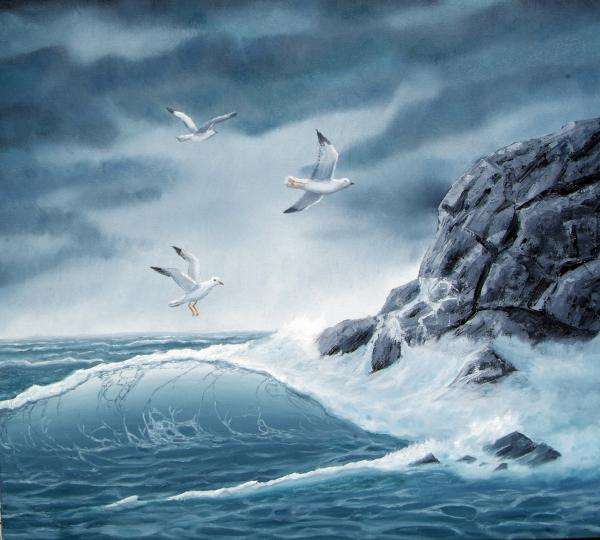
\includegraphics[scale=0.17]{title.jpg}
  \end{center}
\end{figure}
under guidance of\\
Prof. Sudha Shastri\\
IIT Bombay
\end{center}
\end{frame}
\begin{frame}{Outline}
  \begin{multicols}{2}
  \tableofcontents  
  \end{multicols}
\end{frame}
\section{Introduction}
\subsection{A brief history of Colonization}
\begin{frame}{A brief history of British Colonization}
  \begin{columns}[c]
    \column{.6\textwidth}
  \begin{itemize}
  \item \textbf{1492} Columbus discovered America (mistook it for India)
  \item \textbf{1497} Henry VII commissions John Cabot; First Englishman in America
   %No colonization so far, just trade. John Cabot's ship disappeared in his second voyage.
  \item \textbf{1576 onwards} Early claims of land in the name of queen
  \item \textbf{1607} Colonization of America started, with \emph{Virginia Company} creating colony at Jamestown, Virginia
    %Parallels with the colonial discourse prophetic, rather than descriptive
  \end{itemize}
  \column{.4\textwidth}
    \begin{figure}[htp]
      \begin{center}
        \centering
        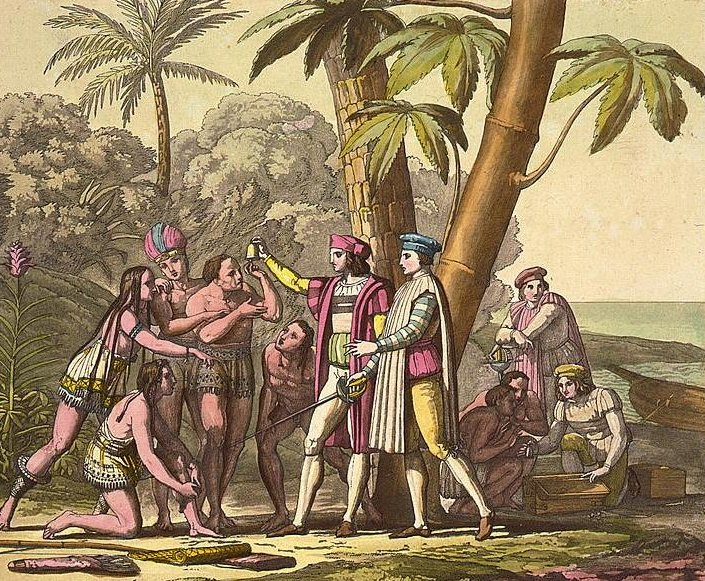
\includegraphics[scale=0.29]{columbus.jpg}
      \end{center}
    \end{figure}
    \end{columns}
\end{frame}

\begin{frame}{The Sea Venture incident}
  \begin{columns}[c]
    \column{.4\textwidth}
    \begin{figure}[htp]
      \begin{center}
        \centering
        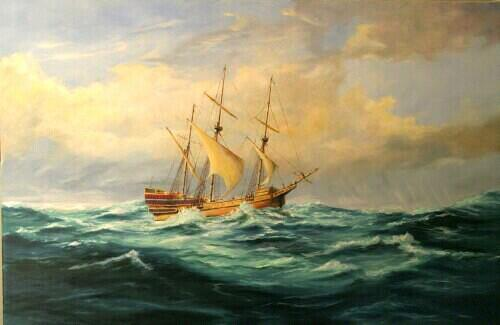
\includegraphics[scale=0.29]{seaventure.jpg}
      \end{center}
    \end{figure}
    \footnotesize{\emph{The Sea Venture in a heavy Sea in 1609,} painting by Christopher Grimes}
    \column{.6\textwidth}

  \begin{itemize}
  \item \emph{Sea Venture} commissioned in 1609 to deliver supplies to the Jamestown colony
  \item Set sail on June 20; Ran into storm and sank on July 24
  \item All 150 passengers land safely ashore, onto a reef in Bermuda
  \item Stranded for 9 months; built 2 new boats; sailed to Virginia; most saved
  \item William Strachey wrote accounts, which supposedly inspired The Tempest
  \end{itemize}
  \end{columns}
\end{frame}

\subsection{The Tempest}
\begin{frame}{The Tempest}
  See video 'The Tempest in a minute'
\end{frame}


\begin{frame}{The Tempest ~\cite{tempest}}
  \begin{itemize}
    \item Shakespeare's last play; written in 1610-11
    \item Based in the Mediterranean, but the island seems more like the \emph{New World}
    \item Strict observation of the three unities, in contrast to other Shakespeare's plays 
    \item Prospero an image of Shakespeare, with his renunciation of magic depicting Shakespeare's farewell to the stage
    \item Colonization had just started, hence parallels with the colonial discourse prophetic, rather than descriptive
  \end{itemize}
\end{frame}

\subsection{The Afterlives}
\begin{frame}{The Afterlives}
  \begin{enumerate}
  \item \textbf{Neil Gaiman's \emph{The Tempest}}~\cite{gaimantempest}
    \begin{itemize}
    \item \textbf{1997} Last book of \emph{The Sandman} series, part of \emph{The Wake}
    \end{itemize}
  \item \textbf{Charles and Mary Lamb's \emph{Tales from Shakespeare} }~\cite{lamb}
    \begin{itemize}
    \item \textbf{1807} Written as an abridged version of Shakespeare for children
    \item Attempts to be a reproduction, but is an afterlife, due to cultural sensibilities of its times
    \end{itemize}
  \item \textbf{The Tempest: Graphic Novel}~\cite{tempestgraphicnovel}
    \begin{itemize}
    \item \textbf{2009} Retains the original text, but adds pictures
    \end{itemize}
  \end{enumerate}
\end{frame}

\section{Postcolonial Theory and The Tempest}
\subsection{Prospero and Postcolonialism}
\begin{frame}{Postcolonial Theory and The Tempest}
  \emph{``Postcolonialism is intellectual discourse that consists of reactions to, and analysis of, the cultural legacy of colonialism and imperialism.''}
  --Harald Fischer-Tine
  \begin{itemize}
    \item The tempest has been viewed through a lens of postcolonial theory
    \item Prospero, earlier seen as a \emph{benevolent God}, has flaws
      \begin{itemize}
      \item Seen as patriarchal, colonialist, sexist and racist
      \item \textbf{Ariel} A companion or familiar. Desires freedom
      \item \textbf{Caliban} A slave. Often mistreated, and used for menial tasks. Justified due to his attempted rape on Miranda
      \item \textbf{Miranda} Prospero's daughter. Prospero is protective, often domineering. Finds it hard to let her go
      \end{itemize}
  \end{itemize}
  \end{frame}
\subsection{Caliban}
  \begin{frame}{Caliban and the Colonial Discourse 1/2}
    \begin{itemize}
    \item Sycorax's son, original inhabitant of the island, at peace with nature; Parallels with Indians
    \item \textcolor{red}{\emph{``And then I lov'd thee, and show'd thee all the qualities o' th' isle .....Cursed be I that did so!.....For I am all the subjects that you have, which first was mine own King''}} (Act 1, Scene 2)
    \item Seen as savage, uncivilized.~\cite{1989} Prospero sees the need to \emph{civilize} him; White man's burden
    \end{itemize}
  \end{frame}
  \begin{frame}{Caliban and the Colonial Discourse 2/2}
    \begin{itemize}
    \item Attempted rape of Miranda \textcolor{red}{\emph{``Would't had been done! Thou didst prevent me; I had peopled else this isle with Calibans''}} (Act 1, Scene 2) Wishes to dominate what he sees are rightfully his own island. Colonizer sees it as a threat to his own dominance, hence subjugates him
    \item \textcolor{red}{\emph{``You taught me language; And my profit on't is, I know how to curse''}} (Act 1, Scene 2); Postcolonial literature often in the colonizer's language, though critical of colonization
    \item Stephano and Trinculo pour wine down his throat and reduce him to a boot-licking slave; Colonization of the worst kind
    \end{itemize}
  \end{frame}

  \begin{frame}{More Caliban}
      Charles Lamb says \textcolor{red}{\emph{``...a strange misshapen thing, far less human in form than an ape.... would have been very kind to him, but the bad nature,.... would not let him learn anything good or useful: therefore he was employed like a slave, to fetch wood, and do the most laborious offices;}}

        The Tempest: Graphic Novel depicts caliban as a non-human, almost demon-like creature. 

        \begin{figure}[htp]
          \begin{center}
            \centering
            \includegraphics[scale=0.02]{caliban1.jpg}
            \includegraphics[scale=0.02]{caliban2.jpg}
          \end{center}
        \end{figure}

        Attempt to dehumanize him, so as to not elicit sympathy, and justify Prospero's conduct. Shakespeare is more neutral, and shows Caliban's POV too.
  \end{frame}

  \subsection{Counterview}
  \begin{frame}{Counterview}
  Meredith Anne Skura ~\cite{1989} says that the Colonial Discourse in \emph{The Tempest} is unintentional. 
  \begin{itemize}
  \item Shakespeare explored exploitation in other plays too; not necessarily in a colonial context
  \item The timeframe when the play was written does not allow for it
  \item Sees the characters as manifestations of human personalities
    \begin{itemize}
    \item \textcolor{red}{\emph{``...this thing of darkness! Acknowledge mine.''}} (Act 5, Scene 1)
    \end{itemize}
  \end{itemize}
  \end{frame}

  \section{Neil Gaiman's The Tempest}
  \subsection{Preliminaries}
  \begin{frame}{Neil Gaiman's The Tempest}
    \begin{itemize}
      \item Neil Gaiman : Comic Books :: Shakespeare : Drama
      \item Last book of the Sandman series ~\cite{gaimanmnd}~\cite{gaimantempest}, last play by Shakespeare, Gaiman sees himself in Shakespeare, Shakespeare sees himself in Prospero
      \item Highlights the labours of writing; writing as a chore instead of it being a creative process
      \item Comments on universality and immortality of Shakespeare
    \end{itemize}
  \end{frame}
  
  \begin{frame}[allowframebreaks]{The Graphic Novel vs The Play}
    Similarities
    \begin{itemize}
    \item Comics have union of verbal and visual presentation, but lack photgraphic realism, thus leaving much to imagination of the viewer
    \item In Elizabethan theater too, minimal use of props meant that the user had to imagine the scene and the setting

      \begin{itemize}
        \item \textcolor{red}{``[c]omics are often compared to film, but I see them as being more like theater, another medium that can't physically show everything and so must rely upon suggestion supported by a few perfectly chosen details''}--Mark Zulli ~\cite{sixcharacters}
      \end{itemize}
    \end{itemize}
    Differences
    \begin{itemize}
    \item \textbf{Omnipresent Narrator} Used extensively by Neil Gaiman; not so much by the other Graphic Novel
      \begin{figure}[htp]
        \begin{center}
          \centering
          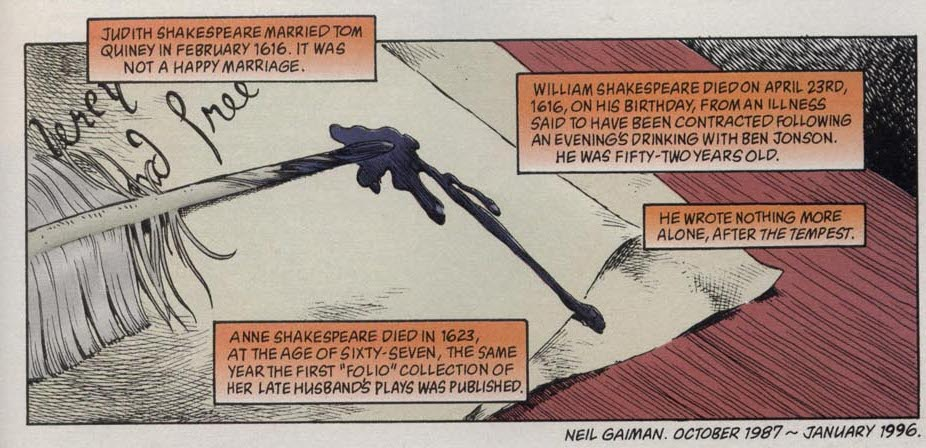
\includegraphics[scale=0.35]{omnipresent.jpg}
        \end{center}
      \end{figure}
    \item \textbf{Font and text styles} Gaiman uses different fonts to suggest differnt moods and people
    \item \textbf{Rapid Scene Changes} Possible in a comic book, but not on stage. Gaiman uses it to juxtapose scenes from The Tempest in scenes from Shakespeare's life
    \end{itemize}
  \end{frame}
  
  
  \begin{frame}{The Afterlife}
    \begin{itemize}
  \item An afterlife may seek to fill in gaps in the original text
  \item Might attempt to explain or justify why certain things are the way they are in the original text
  \item Justification required when the cultural context changes -- e.g. in a postcolonial world
  \item Hob Gadling's (another Sandman character) remorse over slave trade is congruent to Afterlives justifying aspects of the original text
    \end{itemize}
  \end{frame}
  
  \subsection{Themes}
  \begin{frame}{Labours of Writing}
    \begin{columns}[c]
      \column{.6\textwidth}
      \begin{itemize}
      \item The \emph{Furor Poetica}~\cite{gaimanmnd} in contrast to the weary Shakespeare here
      \item Nagging wife, daughter's marriage
      \item Shakespeare writes the play as an obligation to Morpheus; Doesn't quite enjoy writing
      \item Speculation: Was Gaiman bored of the Sandman series by this time? (Not bored of writing; wrote plenty of novels later)
      \item At the end of the book, Morpheus takes away Shakespeare's writing skill. Was the skill never Shakespeare's own, then?
      \end{itemize}
      \column{.4\textwidth}
      \begin{figure}[htp]
        \begin{center}
          \centering
          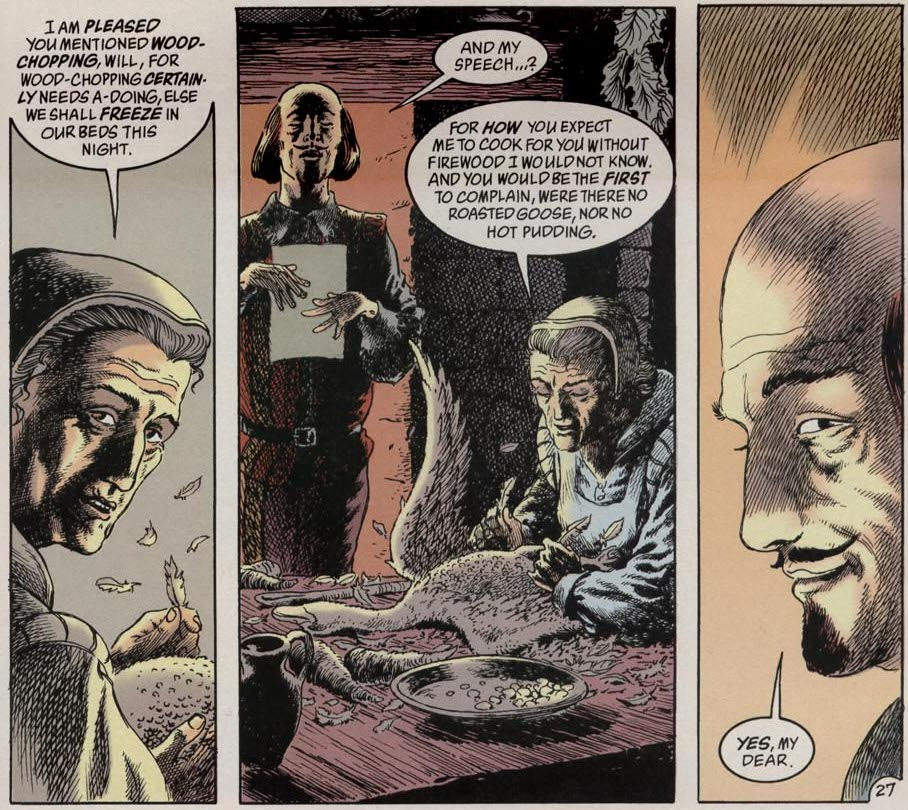
\includegraphics[scale=0.2]{nagging.jpg}
        \end{center}
      \end{figure}
      
      \begin{figure}[htp]
        \begin{center}
          \centering
          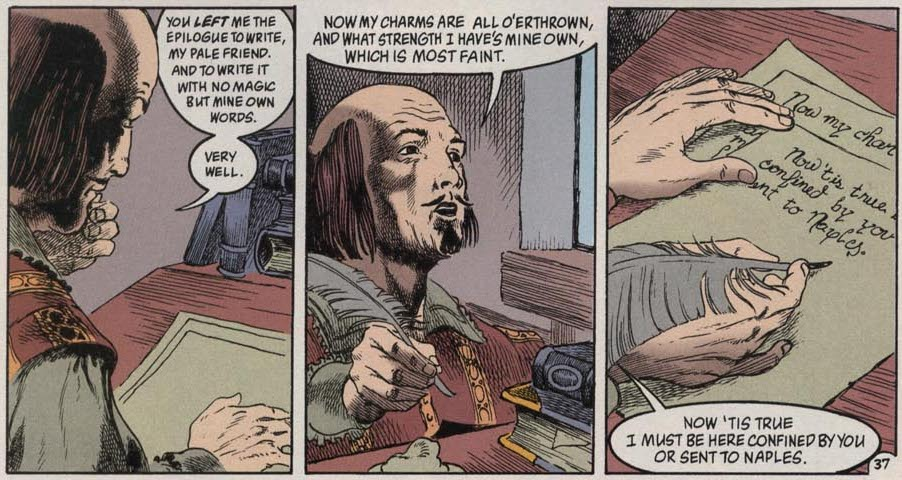
\includegraphics[scale=0.3]{epilogue.jpg}
        \end{center}
      \end{figure}
      
      \end{columns}
    \end{frame}

  \begin{frame}{Shakespeare and Prospero}
    %Discuss parallels between Shakespeare and  Prospero, Judith and Miranda (with pictures)
    \begin{columns}[c]
      \column{.5\textwidth}
      \begin{figure}[htp]
        \begin{center}
          \centering
          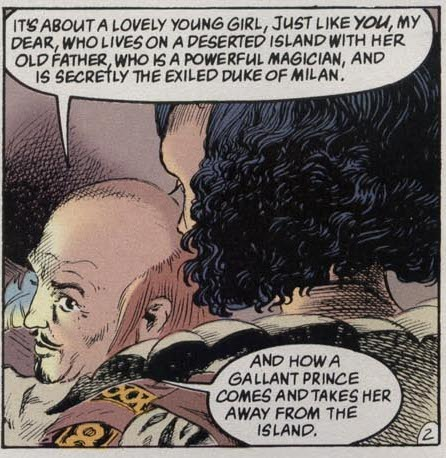
\includegraphics[scale=0.35]{judith.jpg}
          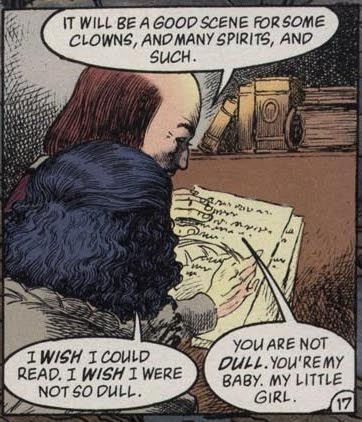
\includegraphics[scale=0.35]{judith2.jpg}
        \end{center}
      \end{figure}
      
      \begin{figure}[htp]
        \begin{center}
          \centering
          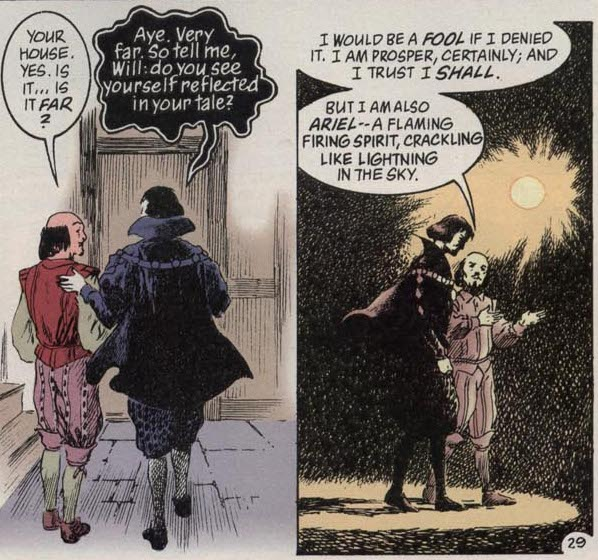
\includegraphics[scale=0.32]{prospere.jpg}
        \end{center}
      \end{figure}
      
      %% \begin{figure}[htp]
      %%   \begin{center}
      %%     \centering
      %%     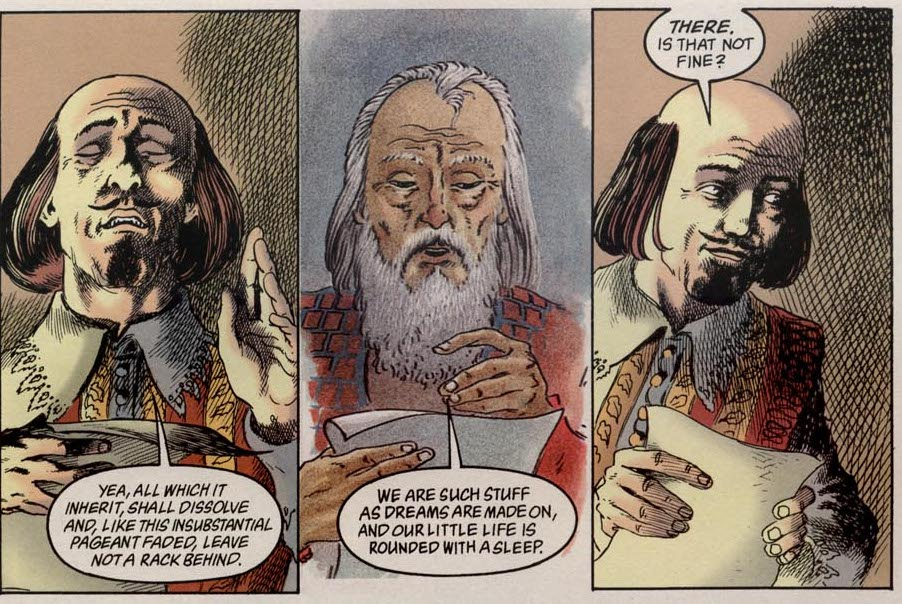
\includegraphics[scale=0.32]{shakespero.jpg}
      %%   \end{center}
      %% \end{figure}

      \column{.5\textwidth}
      \begin{itemize}
      \item Gaiman identifies Prospero as an image of Shakespeare himself
      \item Both love, and feel protective about their daughters; both find it hard to let her go
      \item Prospero renounces his magic; Shakespeare ceases writing
      \end{itemize}
    \end{columns}
  \end{frame}
  
  \begin{frame}{Ben Johnson, and reaction to Shakespeare}

      \begin{figure}[htp]
        \begin{center}
          \centering
          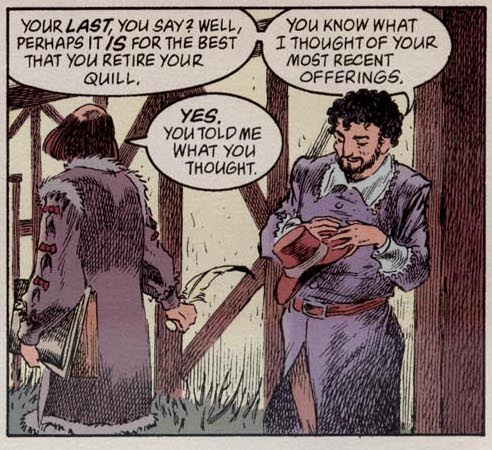
\includegraphics[scale=0.32]{ben.jpg}
          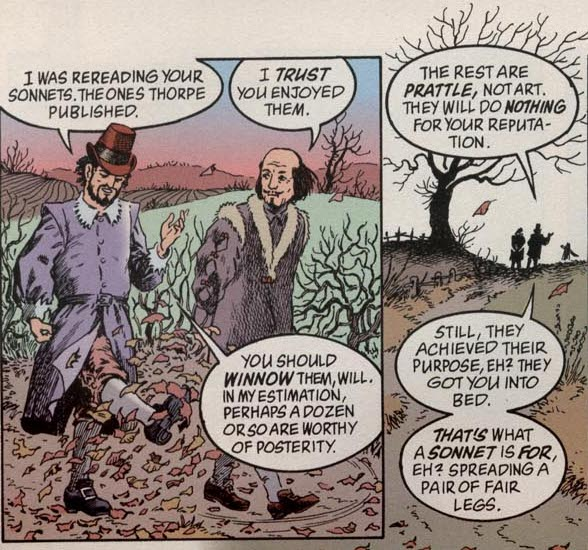
\includegraphics[scale=0.28]{ben2.jpg}
        \end{center}
      \end{figure}
      
      As Gaiman points out, drama was not treated as high art in Shakespeare's time. Though plays were extremely popular, playwrights were seen as not respectable, and ungodly men. Perhaps a commentary on comic books in the present.

      \begin{figure}[htp]
        \begin{center}
          \centering
          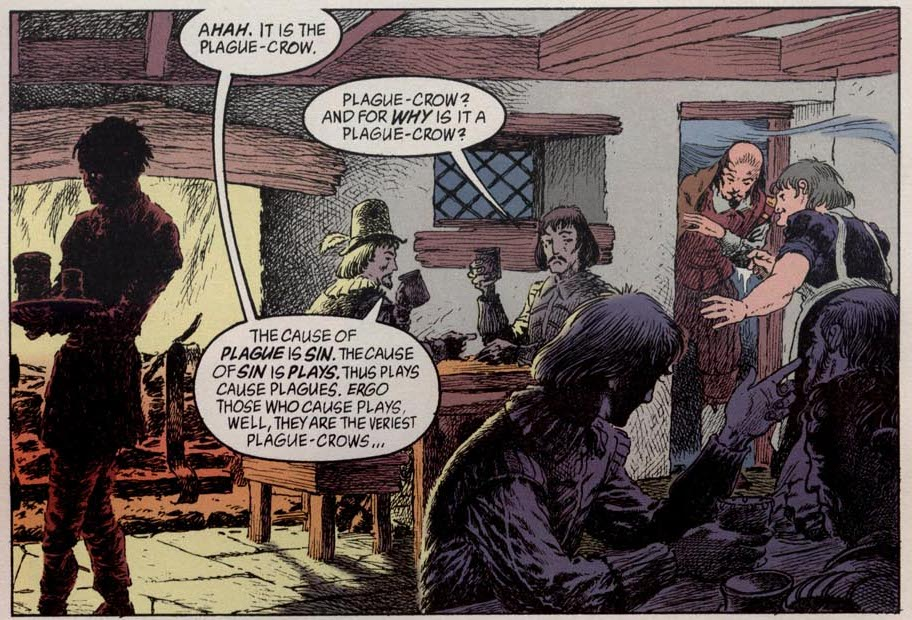
\includegraphics[scale=0.3]{plague.jpg}
        \end{center}
      \end{figure}
      
  \end{frame}
  \subsection{Universality of Shakespeare}
  \begin{frame}{Universality of Shakespeare 1/2}
    \begin{columns}[c]
      \column{.5\textwidth}
      \begin{figure}[htp]
        \begin{center}
          \centering
          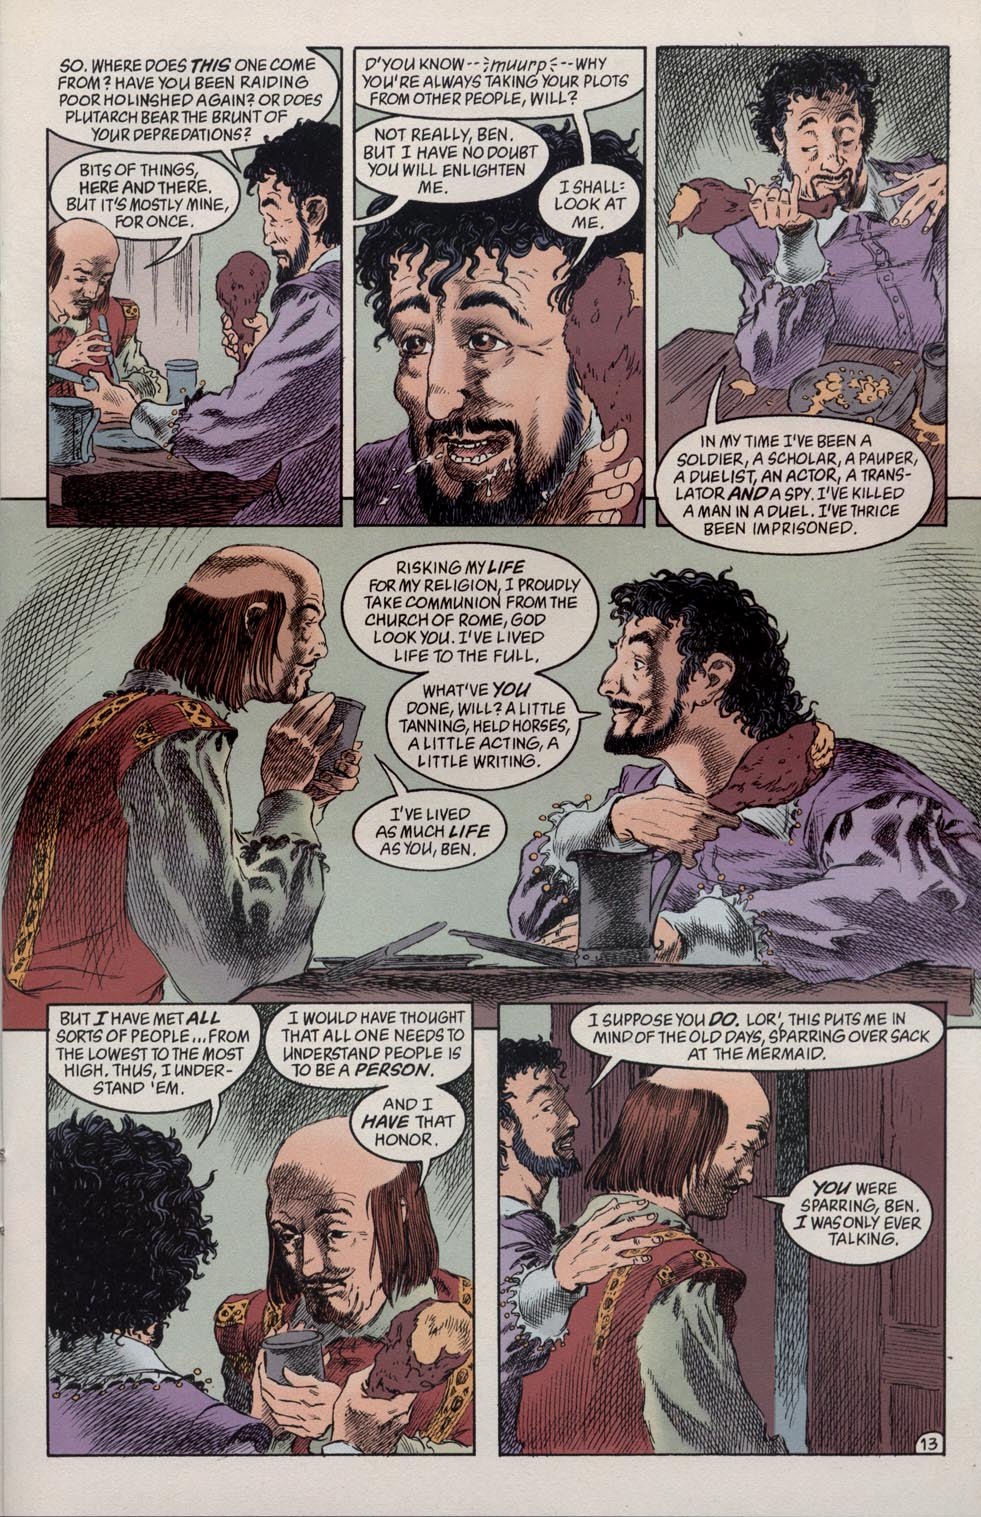
\includegraphics[scale=0.3]{universality.jpg}
        \end{center}
      \end{figure}
      \column{.6\textwidth}
      Johnson feels that one needs to experience different kinds of situations in order to write about them. Shakespeare says, \textcolor{red}{\emph{``All one needs to understand people is to be a person''}}. Gaiman says that this acute understanding of the pulse of human nature and emotions makes Shakespeare so appealing, even today.
    %The conversation with Ben Johnson, in which Shakespeare says that all one needs to appeal to people, is to be a human being, and to understand human emotions.
    %Here, also discuss the Meredith Anne Skura's paper, that says that the parallels to colonization in The Tempest are coincidental, and its all due to Shakespeare's acute understanding of human nature
    \end{columns}
  \end{frame}

  \begin{frame}{Universality of Shakespeare 2/2}
    \begin{itemize}
      \item Did Shakespeare really expect to become immortal, while he lived? According to Gaiman, yes (The Faustian bargain with Morpheus). However, like any other playwright of his time, Shakespeare too was a slave of the quirks of production. 
      \begin{figure}[htp]
        \begin{center}
          \centering
          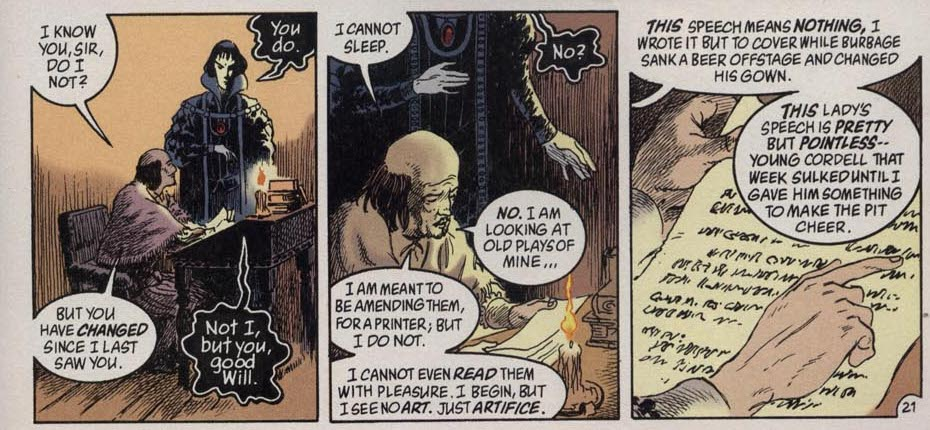
\includegraphics[scale=0.32]{routine.jpg}
        \end{center}
      \end{figure}

    \item Is there really a point to analysing Shakespeare to death, when actually there may not be as much meaning or depth as we think?
      
    \item Is the immortality of Shakespeare a fluke? How much better was he than his contemporaries?
    \end{itemize}
  \end{frame}

  \section{Discussion}
  \begin{frame}{Conclusions and Discussion}
    \begin{enumerate}
    \item Why did Shakespeare decide to strictly follow the 3 unities in this play, when he so easily violated them earlier?
    \item Is Shakespeare really great and worthy of this respect 400 years later? Or was it just a fluke?
    \item On a related note, is Neil Gaiman's supposed greatness also merely a fluke?
    \item Is the colonial discourse in \emph{The Tempest} intentional, or a coincidence?
    \end{enumerate}
  \end{frame}

  \begin{frame}[allowframebreaks]{References}
  \footnotesize{
  \bibliographystyle{abbrv}
  \bibliography{presentation}
  }
  \end{frame}
\end{document}
